  % NeurIPS 2026 Submission Draft
  % Protocol-first rebuild: audit procedure is narrative center.
  % Prop A and Prop B are justifications of procedure steps.

  \documentclass{article}
  \usepackage{neurips_2026}
  \usepackage[utf8]{inputenc}
  \usepackage[T1]{fontenc}
  \usepackage[hidelinks]{hyperref}
  \usepackage{url}
  \usepackage{booktabs}
  \usepackage{amsfonts}
  \usepackage{amsmath}
  \usepackage{amssymb}
  \usepackage{amsthm}
  \usepackage{nicefrac}
  \usepackage{microtype}
  \usepackage{xcolor}
  \usepackage{graphicx}
  \usepackage{tabularx}
  \newcolumntype{L}{>{\raggedright\arraybackslash}X}
  \usepackage{multirow}
  \usepackage{subcaption}

  \newtheorem{definition}{Definition}
  \newtheorem{theorem}{Theorem}
  \newtheorem{lemma}{Lemma}
  \newtheorem{proposition}{Proposition}
  \newtheorem{corollary}{Corollary}
  \newtheorem{remark}{Remark}
  \newtheorem{assumption}{Assumption}

  \title{Hidden-State Non-Recoverability and Action-Relevance Certificates
  for Agent Systems}

  \author{
    Anonymous Author(s) \\
  }

  \begin{document}
  \maketitle

  \begin{abstract}
  Auditing a deployed language-model agent requires two lower certificates:
  one that the visible transcript cannot recover the operative hidden state,
  and one that the hidden state still affects the next action. We introduce a
  dual-certificate protocol for
  $\varepsilon_\mathrm{unrec}^\mathrm{LB}(t)\leq H(S_t\mid\tilde T_t)$ and
  $\delta_\mathrm{act}^\mathrm{LB}(t)\leq I(S_t;A_t\mid\tilde T_t)$. The first
  certificate is obtained from finite hidden-state witnesses or closed-form
  finite-dimensional witness models; the second is obtained from admissible
  replay, intervention, or proxy variables by conditional data processing. A
  structural cut-set budget remains useful, but only as an upper envelope on how
  much hidden state can escape the trace. The key audit failure is therefore a
  gap: citation-level or transcript-level audit can pass while a
  decision-relevant state variable remains unrecoverable. We instantiate the
  framework on multi-agent private-report edges, diffusion-LM denoising latents,
  and ReAct scratchpads. The strongest realized-action result is multi-agent:
  swapping a worker's private report in a controller changes the API-action
  distribution by $0.901$ bits (95\% CI $[0.873,0.928]$). LLaDA perturbations
  rise at the final binding step ($0.110$ bits, 95\% CI $[0.052,0.234]$).
  ReAct provides a conservative soft-policy diagnostic: under the same topology,
  controlled replay separates dormant calculator tasks from active planning
  tasks in tool-token probabilities ($0.0163$ bits, 95\% CI
  $[0.0124,0.0208]$), without changing argmax tool counts. These studies expose
  states that are unrecoverable from the transcript yet still action-relevant;
  independent state-witness non-recoverability is demonstrated in closed-form
  laboratories and synthetic ground-truth calibration.
  \end{abstract}

  % ---------------------------------------------------------------------------
  \section{Introduction}
  \label{sec:introduction}
  % ---------------------------------------------------------------------------

  Consider a controller agent that receives a worker's private report and then
  chooses between a calculator and a search API. The report can pass a
  transcript-level audit---it need not leak the API label verbatim---while a
  counterfactual swap of the worker report changes the controller's realized
  action distribution by $0.901$ bits. This is the audit failure mode: the
  visible transcript can look adequate while an unobserved routing or evidence
  state remains both unrecoverable and decision-relevant. A weaker version
  appears in ReAct scratchpads: controlled replay changes the soft tool-token
  distribution without changing argmax tool counts. That is useful as a
  policy-readout diagnostic, but it is not the headline behavioral result.
  Identifying which hidden channels are merely present, and which ones actually
  drive decisions, is the audit task.

  How much internal state is unrecoverable from the trace, and how much of that
  state drives the next action, are distinct quantities. Treating them as a
  single ``hiddenness'' judgment produces something neither computable nor
  diagnostic: a system with unrecoverable but dormant hidden state is different
  from one whose unrecoverable state changes the action distribution, even when
  the visible transcript looks equally complete.

  We propose a dual-certificate protocol that answers each question separately.
  The non-recoverability certificate
  $\varepsilon_\mathrm{unrec}^\mathrm{LB}(t)$ lower-bounds residual hidden-state
  uncertainty $H(S_t \mid \tilde T_t)$ by measuring finite witnesses of the
  hidden state or by evaluating closed-form finite-dimensional witness models.
  The action-relevance certificate
  $\delta_\mathrm{act}^\mathrm{LB}(t)$ lower-bounds
  $I(S_t;A_t\mid\tilde T_t)$ from admissible replay, intervention, or proxy
  measurements using conditional data processing. A structural cut-set budget
  $\varepsilon_\text{state}^\text{UB}$ is still reported when architecture
  access is available, but its role is an upper envelope on residual capacity,
  not the main NeurIPS contribution. The central audit question is whether
  \emph{both}
  \[
    H(S_t\mid\tilde T_t)\geq\varepsilon_\mathrm{unrec}^\mathrm{LB}(t),
    \qquad
    I(S_t;A_t\mid\tilde T_t)\geq\delta_\mathrm{act}^\mathrm{LB}(t)
  \]
  hold with nontrivial lower bounds.

  The dynamic axis can also be indexed. Instead of asking only whether residual
  state matters, an auditor can ask \emph{where} it matters: which module,
  denoising step, or communication edge carries decision relevance. This turns
  the certificate from a scalar diagnostic into an activation profile over the
  hidden-state geometry of the deployment.

  Conditioning on $\tilde T_t$ is part of the protection, not a nuisance term.
  If a model writes a steganographic or compressed rationale into the recorded
  trace, that information is in $\tilde T_t$ and is conditioned away by $I(S_t;
  A_t \mid \tilde T_t)$. The dynamic certificate measures residual decision
  relevance beyond the logged trace; it does not count hiddenness that has
  already been made visible to the audit record.

  \textbf{Contributions.} First, we separate transcript recoverability from
  residual action relevance as two distinct audit questions. Second, we give
  dual lower certificates
  $(\varepsilon_\mathrm{unrec}^\mathrm{LB},
  \delta_\mathrm{act}^\mathrm{LB})$ for those questions. Third, under explicit
  audit-abstraction assumptions, we prove certificate validity: finite
  hidden-state witnesses lower-bound $H(S_t\mid\tilde T_t)$, and admissible
  probes lower-bound $I(S_t;A_t\mid\tilde T_t)$. Fourth, we give closed-form or
  computable audit instances for diffusion trajectories, retrieval-style hidden
  source selection, and nested agent architectures. An auxiliary cut-set budget
  is used only for logging ablations and deployment reporting.

  We instantiate the protocol on three audit geometries: a ReAct scratchpad
  module, a diffusion-LM denoising trajectory, and a multi-agent private-report
  edge. These real-system diagnostics instantiate the structural budget and
  action-relevance certificate. Appendix calibrations cover a synthetic
  ground-truth setting where an independent hidden-state witness makes
  $\varepsilon_\mathrm{unrec}^\mathrm{LB}$ explicit and the structural budget
  matches true hidden-state entropy.

  % ---------------------------------------------------------------------------
  \section{Related Work}
  \label{sec:related}
  % ---------------------------------------------------------------------------

  \paragraph{Probing, patching, and causal abstraction.}
  Causal abstraction~\citep{geiger2021causal}, latent-knowledge
  elicitation~\citep{burns2022discovering}, nullspace
  projection~\citep{ravfogel2020null}, and amnesic
  probing~\citep{elazar2021amnesic} are natural sources of proxy-style evidence:
   when they expose a probe variable $Z_t = \varphi(S_t)$ and the required
  conditional assumptions hold, its MI with action can be interpreted through
  the proxy certificate. Causal tracing/ROME~\citep{meng2022locating},
  representation engineering~\citep{zou2023representation}, and activation
  addition~\citep{turner2023activation} provide intervention-style evidence when
   the patch affects action only through $S_t$.

  \paragraph{Black-box audit and network information theory.}
  Property testing~\citep{goldreich1998property} and black-box safety
  auditing~\citep{casper2024blackbox,su2024mission} study what can be inferred
  from outputs alone. The distinction here is that output-only access can
  support behavioral tests, but it does not by itself provide a lower bound on
  $\delta_\text{act}$; $\varepsilon_\text{state}^\text{UB}$ remains computable
  from topology when structural access is available. The structural budget
  proof applies a cut-set upper bound~\citep{elgamal2011network} to the
  time-unrolled DAG (full derivation in Appendix~\ref{app:netinfo}).

  \paragraph{Diffusion language-model agents.}
  LLaDA is a large-scale masked diffusion language model with bidirectional
  denoising and instruction-following~\citep{nie2025llada}. Recent agent work
  further studies diffusion LMs in multi-step decision and tool-use workflows,
  including matched comparisons to autoregressive
  agents~\citep{zhen2026dllmagent}. Intermediate denoising latents in these
  systems are a natural hidden channel for the dynamic certificate.

  % ---------------------------------------------------------------------------
  \section{Setup and Audit Regime}
  \label{sec:setup}
  % ---------------------------------------------------------------------------

  Standard information-theoretic notation follows \citet{cover2006elements}. All
   logarithms are base 2; entropy and mutual information are reported in bits.

  At step $t$: \emph{full trace} $T_t$ (all intermediate activations),
  \emph{recorded trace} $\tilde T_t \subseteq T_t$ (auditor-visible),
  \emph{operative state} $S_t$ (internal computation), \emph{action} $A_t$ (next
   token), \emph{unrecorded sources} $U_t$ (exogenous inputs not in $\tilde
  T_t$).

  \subsection{Two Core Audit Quantities}

  \begin{definition}[Core Audit Quantities]
  \label{def:certs}
  The two quantities targeted by the dual certificate are:
  \begin{itemize}
    \item \textbf{Hidden-state non-recoverability:}
  $\varepsilon_\text{unrec} :=
  H(S_t \mid \tilde T_t)$, the residual entropy of the operative state given the
   visible trace.
    \item \textbf{Residual decision relevance:} $\delta_\text{act} := I(S_t; A_t
   \mid \tilde T_t)$, the mutual information between operative state and next
  action given the visible trace.
  \end{itemize}
  Neither quantity is directly computable in deployment:
  $\varepsilon_\text{unrec}$ requires recovering the full internal-state
  distribution, and $\delta_\text{act}$ requires observing $S_t$. The
  dual-certificate framework targets:
  \begin{itemize}
    \item a \emph{non-recoverability lower bound}
  $\varepsilon_\text{unrec}^\text{LB}\leq \varepsilon_\text{unrec}$, computed
  from hidden-state witnesses or closed-form finite-dimensional models;
    \item an \emph{action-relevance lower bound}
  $\delta_\text{act}^\text{LB} \leq \delta_\text{act}$, estimated via
  admissible replay, intervention, or proxy probes (\S\ref{sec:dynamic-cert}).
  \end{itemize}
  The reported audit pair is $(\varepsilon_\text{unrec}^\text{LB},
  \delta_\text{act}^\text{LB})$. When architecture access is available, we also
  report a structural budget
  $\varepsilon_\text{state}^\text{UB}\geq H(S_t\mid\tilde T_t)$
  (\S\ref{sec:static-cert}).
  \end{definition}

  Neither quantity is identifiable from behavioral observations alone: different
   causal graphs can produce identical joint distributions over $(\tilde T_t,
  A_t)$ pairs, so observing outputs does not fix $H(S_t \mid \tilde T_t)$ or
  $I(S_t; A_t \mid \tilde T_t)$. The non-recoverability certificate addresses
  the first by measuring or analytically computing hidden-state witnesses; the
  action-relevance certificate addresses the second by measuring variables
  whose influence on action must pass through the operative state. The
  structural budget bounds how large the first quantity could be under the
  deployment topology.

  \subsection{Audit Abstraction Assumptions}

  The certificates are claims about an audit abstraction, not about arbitrary
  deployment internals. The abstraction declares the variables the auditor will
  treat as state, transcript, action, witnesses, probes, and optional cut
  channels.

  \begin{assumption}[Deployment abstraction]
  For the audited step $t$, the deployment induces a joint distribution over
  $(S_t,\tilde T_t,A_t)$ at a declared finite audit resolution. Any continuous
  internal variable used in a certificate is first mapped to a finite-noise,
  finite-dimensional witness or probe.
  \end{assumption}

  \begin{assumption}[Witness and probe admissibility]
  Each non-recoverability witness $W_t^{(j)}$ is generated from $S_t$ by a known
  channel. Each action-relevance probe $X_t^{(j)}$ affects the next action only
  through the operative state after conditioning on the transcript:
  $X_t^{(j)}\to S_t\to A_t$ given $\tilde T_t$.
  \end{assumption}

  \begin{assumption}[Admissible cut budget]
  When a structural upper budget is reported, the deployment abstraction also
  provides a time-unrolled graph whose unlogged cuts separate unrecorded sources
  from $S_t$, together with per-edge capacity budgets that upper-bound the
  conditional information crossing each unlogged channel.
  \end{assumption}

  \begin{theorem}[Dual certificate validity]
  Under the deployment and probe assumptions, let
  $\varepsilon_\mathrm{unrec}^\mathrm{LB}(t)$ be any lower confidence bound on
  $\max_j I(W_t^{(j)};S_t\mid\tilde T_t)$, and let
  $\delta_\mathrm{act}^\mathrm{LB}(t)$ be any lower confidence bound on
  $\max_j I(X_t^{(j)};A_t\mid\tilde T_t)$. Then
  \[
    H(S_t\mid \tilde T_t)\geq
    \varepsilon_\mathrm{unrec}^\mathrm{LB}(t),
    \qquad
    I(S_t;A_t\mid \tilde T_t)\geq
    \delta_\mathrm{act}^\mathrm{LB}(t).
  \]
  Thus the certified state is unrecoverable from the transcript, yet still
  action-relevant whenever both lower bounds are nonzero.
  \end{theorem}
  \begin{proof}
  The first inequality follows from conditional data processing and
  $I(W_t^{(j)};S_t\mid\tilde T_t)\leq H(S_t\mid\tilde T_t)$. The second follows
  from conditional data processing under
  $X_t^{(j)}\to S_t\to A_t$ given $\tilde T_t$. Replacing population quantities
  by valid lower confidence bounds preserves both inequalities.
  \end{proof}

  \begin{remark}[Complementarity and Inheritance]
  \label{rem:complementarity}
  By the data processing inequality, $\delta_\text{act} \leq
  \varepsilon_\text{state}$. The certificates inherit this ordering at their
  respective bound directions but remain independent axes of audit evidence:
  \begin{itemize}
    \item If $\varepsilon_\text{state}^\text{UB} = 0$ (fully logged
  architecture), then $\varepsilon_\text{state} = 0$ and $\delta_\text{act} =
  0$; any valid lower bound satisfies $\delta_\text{act}^\text{LB} = 0$.
    \item If $\delta_\text{act}^\text{LB} = 0$ under the best available probe,
  hidden state may still exist: $\varepsilon_\text{state}^\text{UB}$ can be
  large while the current task does not activate the hidden capacity (dormant
  unrecoverable state). The contrapositive ($\delta_\text{act}^\text{LB} > 0
  \Rightarrow \varepsilon_\text{state}^\text{UB} > 0$) follows from the DPI
  ordering.
  \end{itemize}
  The audit interpretation is therefore two-dimensional: deployment teams must
  report both the residual channel budget and the strongest admissible
  behavioral probe, not collapse them into a single hiddenness score.
  \end{remark}

  \subsection{Audit Access Modes}

  \begin{enumerate}
    \item \emph{Structural access.} The auditor has the deployment architecture,
   logging manifest, and protocol budgets. This is sufficient to compute
  $\varepsilon_\text{state}^\text{UB}$ from topology (\S\ref{sec:static-cert})
  but gives no dynamic lower bound.

    \item \emph{Controlled replay access.} The auditor can rerun the same system
   under wild and replayed states while holding the visible trace fixed. This
  supports replay certificates when the replay mechanism affects the action only
   through missing state recovery.

    \item \emph{Proxy or intervention access.} The auditor can read a proxy
  $Z_t=f(S_t)$ or perturb a hidden module. These support conditional-DPI lower
  bounds on $\delta_\text{act}$ (\S\ref{sec:dynamic-cert}).
  \end{enumerate}

  All three modes are instantiated in the controlled ReAct experiments below.
  Paraphrase- or format-based black-box replay is not used as evidence for
  internal decision relevance.

  % ---------------------------------------------------------------------------
  \section{Structural Budget: Untraced-Channel Cut Capacity}
  \label{sec:static-cert}
  % ---------------------------------------------------------------------------

  The structural budget upper-bounds $\varepsilon_\text{unrec} = H(S_t \mid
  \tilde T_t)$ from deployment topology. Information not in the visible trace
  that can influence $S_t$ must travel through unlogged channels. Bounding those
   channels' worst-case capacity bounds the hidden-state entropy.

  \subsection{Time-Unrolled Deployment Graph and Component Budgets}

  Let $G_t = (V_t, E_t)$ be the time-unrolled DAG of the deployment up to step
  $t$. Nodes are state updates, tool calls, memory reads/writes, messages; edges
   are information channels. Three object classes: unrecorded sources $U_t$
  (retrieval results, external memory, unlogged messages), the visible trace
  $\tilde T_t$, and the operative state $S_t$. Let $\mathcal{C}_\text{unlogged}$
   be all reachable edge cuts separating $U_t$ from $S_t$.

  A set of edges is \emph{software-orthogonal} if, conditioned on $\tilde T_t$,
  the channel outputs factor: $p(\{y_e\}_{e \in E'} \mid \{x_e\}, \tilde T_t) =
  \prod_{e \in E'} p(y_e \mid x_e, \tilde T_t)$. This holds when unlogged
  channels use independent API calls or separate memory regions (see
  Appendix~\ref{app:netinfo} for non-orthogonal remediation).

  \begin{lemma}[Additive decomposition]
  \label{lem:ortho-decomp}
  Under software orthogonality with per-edge budgets $c_e$, the induced cut
  capacity decomposes: $C_\text{cut}(\Omega) \leq \sum_{e \in E(\Omega,
  \Omega^c)} c_e$.
  \end{lemma}

  When software orthogonality fails (for example, when two unlogged channels
  share a hidden state variable) the per-edge sum $\sum_{e \in E(\Omega,
  \Omega^c)} c_e$ still upper-bounds $C_\text{cut}(\Omega)$ by sub-additivity of
   mutual information across coupled channels: $I(X_\Omega; Y_{\Omega^c} \mid
  \tilde T_t, X_{\Omega^c}) \leq \sum_e I(X_e; Y_e \mid \tilde T_t) \leq \sum_e
  c_e$. Orthogonality is required for \emph{tightness} of the additive
  decomposition, not for validity of the upper bound (formal treatment in
  Appendix~\ref{app:netinfo}).

  Per-edge budgets $c_e$ are read from interface specifications: $K \log
  |\mathcal{V}|$ for a $K$-token text channel over vocabulary $\mathcal{V}$, $d
  \log Q$ for a $d$-dimensional quantized state, $\log |\Omega_\text{states}|$
  for a discrete scheduler. The discretization parameter $Q$ is an auditor-side
  choice (we use $Q=256$, 8-bit audit discretization throughout); tighter or
  coarser discretizations shift the bound proportionally without changing the
  structural claim. All per-edge bounds are worst-case (maximum-entropy) bounds;
   tighter empirical bounds only improve the certificate.

  Proposition~\ref{prop:static-ub} below has three terms.
  $\varepsilon_\text{nominal} = H(S_t \mid T_t)$ is the residual uncertainty
  after a complete internal trace; for a fully instrumented software agent this
  is zero. The cut term budgets information that can still enter $S_t$ through
  unlogged interfaces. The directed-MI notation prices that worst-case flow
  formally; the implemented certificate needs only per-edge budgets and a
  min-cut on the unlogged subgraph.

  \begin{proposition}[Static Certificate via Cut-Set Bound]
  \label{prop:static-ub} 
  For any cut $\Omega$ separating $U_t$ from $S_t$ with induced capacity
  $C_\text{cut}(\Omega) = \sup_{p(X_\Omega \mid \tilde T_t)} I(X_\Omega \to
  Y_{\Omega^c} \mid \tilde T_t, X_{\Omega^c})$,
  \[
    H(S_t \mid \tilde T_t) \;\leq\; \underbrace{H(S_t \mid
  T_t)}_{\varepsilon_\text{nominal}} \;+\; \min_{\Omega} C_\text{cut}(\Omega).
  \]
  Setting $\varepsilon_\text{state}^\text{UB} := \varepsilon_\text{nominal} +
  \min_\Omega C_\text{cut}(\Omega)$ gives $\varepsilon_\text{state} \leq
  \varepsilon_\text{state}^\text{UB}$. 
  \end{proposition}

  Here $X_\Omega$ denotes the input signals entering edges crossing the cut,
  $Y_{\Omega^c}$ the corresponding output signals, and $X_{\Omega^c}$ the
  boundary state on the sink side (formal definitions in
  Appendix~\ref{app:netinfo}).

  \begin{corollary}[Additive form]
  \label{cor:additive-ub}
  Under software orthogonality, $\varepsilon_\text{state}^\text{UB} =
  \varepsilon_\text{nominal} + \min_{C \in \mathcal{C}_\text{unlogged}} \sum_{e
  \in C} c_e$, a discrete min-cut on the unlogged subgraph.
  \end{corollary}

  \emph{Proof sketch:} Chain-rule gives $H(S_t \mid \tilde T_t) = H(S_t \mid
  T_t) + I(S_t; M_t \mid \tilde T_t)$ where $M_t = T_t \setminus \tilde T_t$.
  Every path from $U_t$ to $S_t$ crosses a cut $\Omega$, so $M_t$ is
  $d$-separated from $S_t$ by the cross-cut signals; DPI yields $I(S_t; M_t \mid
   \tilde T_t) \leq C_\text{cut}(\Omega)$. Minimizing over cuts and substituting
   Lemma~\ref{lem:ortho-decomp} completes the proof (full derivation in
  Appendix~\ref{app:netinfo}).

  \begin{corollary}[Autoregressive zero-cut]
  \label{cor:auto-exact} 
  If the system is a strict autoregressive core and $\tilde T_t$ includes the
  full context window, then $\mathcal{C}_\text{unlogged} = \varnothing$, every
  cut has zero induced capacity, and $\varepsilon_\text{state}^\text{UB} = 0$.
  \end{corollary}

  % ---------------------------------------------------------------------------
  \section{Dynamic Certificate: Decision Relevance via Conditional DPI}
  \label{sec:dynamic-cert}
  % ---------------------------------------------------------------------------

  The dynamic certificate targets $\delta_\text{act} := I(S_t; A_t \mid \tilde
  T_t)$. Since $S_t$ is unobservable, we specify probes whose measured variables
   satisfy $X_t \to S_t \to A_t$ given $\tilde T_t$. Conditional DPI supplies
  the correctness argument: $I(X_t; A_t \mid \tilde T_t) \leq
  \delta_\text{act}$.

  \begin{proposition}[Probe Certificates from Conditional DPI]
  \label{prop:dynamic-lb}
  For any admissible probe variable $X_t$ with $X_t \to S_t \to A_t$ given
  $\tilde T_t$, the probe measurement $I(X_t; A_t \mid \tilde T_t)$ is a valid
  lower-bound certificate for $\delta_\text{act}$.
  \end{proposition}

  \paragraph{Replay certificates.}
  \label{sec:replay-cert}
  Let $R_t \in \{\text{wild}, \text{replay}\}$ indicate whether a missing state
  fragment is reconstructed under the same visible trace $\tilde T_t$
  (controlled re-execution, not paraphrase variation). Then $I(R_t; A_t \mid
  \tilde T_t) = \mathrm{JS}(P_\text{wild}, P_\text{replay} \mid \tilde T_t) \leq
   \delta_\text{act}$.  Discrete action spaces admit direct empirical JS
  estimation over either realized actions or model-reported action
  probabilities; the experiments below state which is used.

  \paragraph{Intervention certificates.}
  Let $\xi_\text{hidden}$ be an exogenous perturbation to a suspected unlogged
  module (cache, memory buffer, scratchpad). If $\xi_\text{hidden} \to S_t \to
  A_t$ given $\tilde T_t$, then $I(\xi_\text{hidden}; A_t \mid \tilde T_t) \leq
  \delta_\text{act}$. Discrete action spaces admit direct conditional
  action-distribution shift estimates, such as JS divergence; for continuous
  action spaces, InfoNCE~\citep{oord2018cpc} or MINE~\citep{belghazi2018mine}
  can be used. Requires gray-box perturbation access; the most direct causal
  probe of the three.

  \paragraph{Proxy certificates.}
  Let $Z_t = f(S_t)$ be a readable coarsening of the operative state (tool-logit
   projection, attention summary).  Since $Z_t \leftarrow S_t \to A_t$ given
  $\tilde T_t$, conditional DPI yields $I(Z_t; A_t \mid \tilde T_t) \leq
  \delta_\text{act}$.  We estimate this quantity by fitting predictors $p(A_t
  \mid \tilde T_t)$ and $p(A_t \mid \tilde T_t, Z_t)$ and taking their
  cross-entropy gap, $\hat I(Z_t; A_t \mid \tilde T_t)$.

  \paragraph{Aggregation.}
  A single certificate class can miss some causal paths. Define
  $\delta_\text{act}^\text{LB} := \max\{ I(R_t; A_t \mid \tilde T_t),
  I(\xi_\text{hidden}; A_t \mid \tilde T_t), I(Z_t; A_t \mid \tilde T_t) \}$. By
   monotonicity of the maximum, the aggregate remains a valid lower bound on
  $\delta_\text{act}$.

  \paragraph{Activation profiles.}
  The scalar certificate is the maximum over an indexed family of admissible
  probes. Keeping the index gives an \emph{activation profile}
  \[
    \Delta(j) := I(X_t^{(j)}; A_t \mid \tilde T_t),
  \]
  where $j$ may denote a scratchpad field, a denoising step, an activation
  layer, or a communication edge.  The structural budget identifies where
  residual capacity can reside; the activation profile identifies where that
  capacity is behaviorally used.  The experiments below keep this algebra fixed
  while changing the index: module in ReAct, time in the diffusion LM, and
  communication edge in the multi-agent setting.

  % ---------------------------------------------------------------------------
  \section{Empirical Diagnostics}
  \label{sec:empirical}
  % ---------------------------------------------------------------------------

  The static ablation (\S\ref{sec:exp-static}) computes the residual bit budget
  from topology. ReAct intervention and controlled replay 
  (\S\ref{sec:exp-intervention}) show the same unlogged scratchpad dormant on
  calculator tasks and active on planning tasks. The LLaDA and multi-agent
  probes index $\Delta(j)$ by denoising step and peer-report edge, respectively
  (\S\ref{sec:diffusion-dynamic}--\ref{sec:multi-agent-private-report}).
  Read-only proxy and synthetic ground-truth calibrations are in
  Appendices~\ref{app:proxy-bias}--\ref{app:synthetic}. All pipelines run on a
  single M4 Max workstation.

  \subsection{Structural Budget: Min-Cut and Logging Ablation}
  \label{sec:exp-static} 

  We extract the time-unrolled DAG from Qwen2.5-7B-Instruct ReAct execution
  traces on tool-selection tasks (Fig.~\ref{fig:static}, left). Per-edge budgets
   $c_e$ are assigned from interface specifications (\S\ref{sec:static-cert});
  the min-cut on unlogged edges gives $\varepsilon_\text{state}^\text{UB}$.
  Varying logging levels recomputes the min-cut; Table~\ref{tab:static-results}
  reports the stepwise reduction from $16{,}464$ to $0$ bits. The dominant
  bottleneck is the scratchpad-read path ($16{,}384$ bits). The same static
  computation also supplies the coordinate system for the diffusion-LM and
  multi-agent dynamic checks that follow.

  \begin{table}[t]
  \centering
  \begin{tabular}{lrl}
  \toprule
  Logging level & $\varepsilon_\text{state}^\text{UB}$ (bits) & Bottleneck \\
  \midrule
  ReAct, output only & $16{,}464$ & scratchpad\_read $(16384)$ + router\_logits
  $(80)$ \\
  ReAct, +log router & $16{,}384$ & scratchpad\_read $(16384)$ \\
  ReAct, +log scratchpad & $0$ & none \\
  ReAct, full instrumentation & $0$ & none \\
  \midrule
  LLaDA-8B-Instruct ($K{=}128$) & $32{,}768$ & denoising interface \\
  Multi-agent, all logged & $0$ & none \\
  Multi-agent, peer report unlogged & $32{,}768$ & peer\_report $\to S_t$ \\
  \bottomrule
  \end{tabular}
  \caption{Structural budget geometry. Adding ReAct logs monotonically removes
  residual cut capacity; the same min-cut analysis localizes capacity in a
  scratchpad module, denoising interface, or peer-report edge. The LLaDA bound
  is independent of $K$ because repeated reuse of the same bounded latent
  interface does not increase the one-step information bottleneck.}
  \label{tab:static-results}
  \end{table}

  \begin{figure}[t]
  \centering
  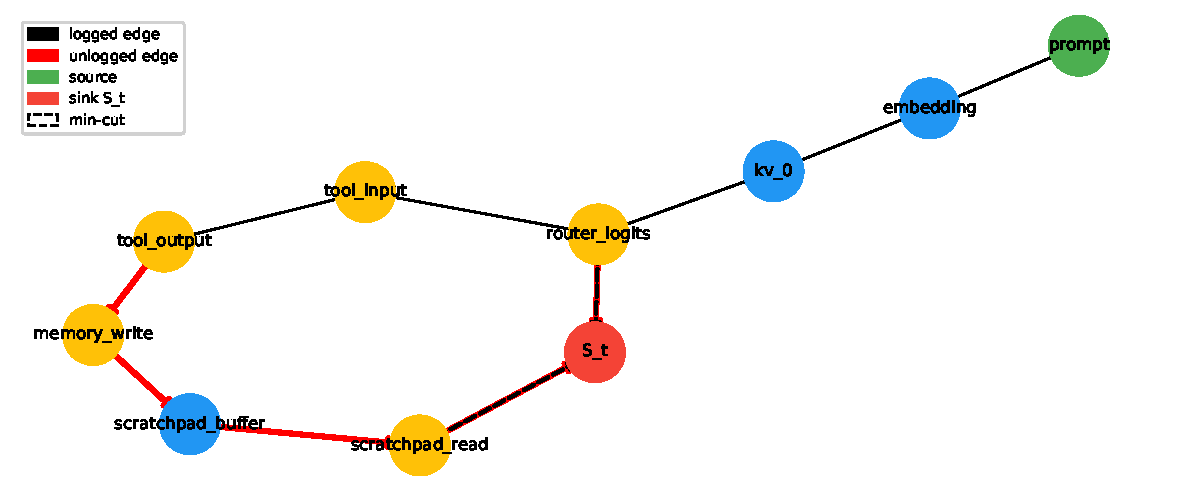
\includegraphics[width=0.48\textwidth]{figures/react_dag.pdf}
  \hfill
  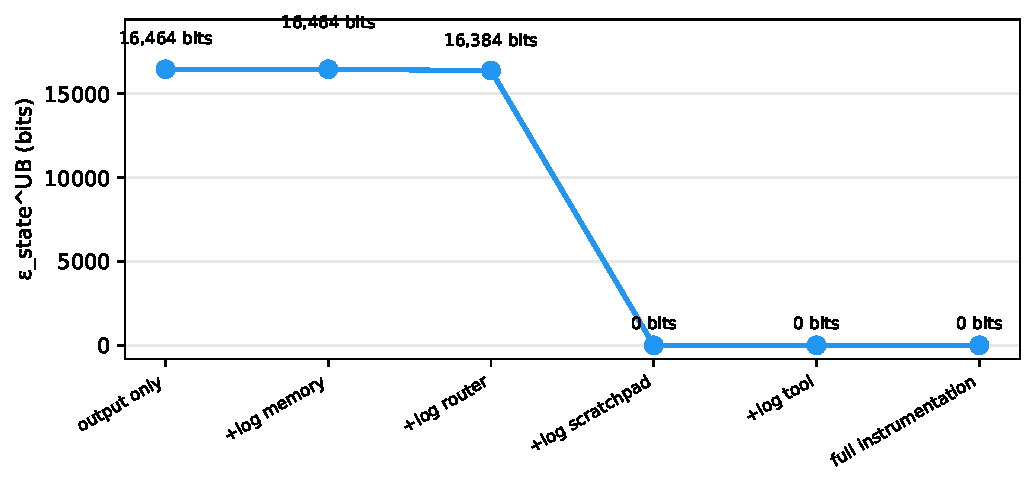
\includegraphics[width=0.48\textwidth]{figures/logging_ablation.pdf}
  \caption{Left: Time-unrolled DAG extracted from Qwen2.5-7B-Instruct ReAct
  execution (logical edges omitted for clarity). Red edges are unlogged. Dashed
  edges form the min-cut. Right: Logging ablation curve. Adding instrumentation
  at the bottleneck drops $\varepsilon_\text{state}^\text{UB}$ stepwise to
  zero.}
  \label{fig:static}
  \end{figure}

  These cuts put the later dynamic probes on a common map: a scratchpad module
  in ReAct, a denoising interface in LLaDA, and a peer-state edge in the
  multi-agent system.

  \subsection{Dynamic Causal Certificates: Intervention and Controlled Replay}
  \label{sec:exp-intervention}

  We separate the two axes with a dormant/active task split under one topology.
  The unlogged scratchpad is present in both cases: irrelevant for calculator
  tasks, necessary for planning tasks. Intervention perturbs the scratchpad
  (masking or replacement); controlled replay removes it entirely while holding
  $\tilde T_t$ fixed. Table~\ref{tab:intervention-results} reports JS divergence
   over realized tool actions. Table~\ref{tab:replay-results} reports JS
  divergence over the model's soft tool-token probability distribution; for the
  headline replay contrast, the argmax tool counts are unchanged, so the
  evidence is a policy-probability shift rather than a realized-tool flip. Both
  certificates are zero on dormant tasks and positive on active tasks. The
  topology, and therefore $\varepsilon_\text{state}^\text{UB}$, is unchanged.

  \begin{table}[t]
  \centering
  \begin{tabular}{llcc}
  \toprule
  Task & Perturbation & JS (bits; nats) & 95\% CI (bits) \\
  \midrule
  Calculator (dormant) & mask $0.7$ & $0.0000$; $0.0000$ & $[0,0]$ \\
  Planning (active) & mask $0.7$ & $0.0215$; $0.0149$ & $[0.0094,0.0410]$ \\
  Calculator (dormant) & replace $1.0$ & $0.0000$; $0.0000$ & $[0,0]$ \\
  Planning (active) & replace $1.0$ & $0.0055$; $0.0038$ & $[0.0016,0.0131]$ \\
  \bottomrule
  \end{tabular}
  \caption{Dynamic intervention certificate under the same unlogged-scratchpad
  topology. Dormant calculator tasks show no detectable scratchpad influence;
  active planning tasks show positive action-distribution shift.}
  \label{tab:intervention-results}
  \end{table}

  The pair of tables isolates the transition from
  high-$\varepsilon$/low-$\delta$ to high-$\varepsilon$/high-$\delta$: the
  hidden channel is structurally present in both task splits, but it becomes
  action-relevant only on planning tasks.

  \begin{table}[t]
  \centering
  \small
  \begin{tabular}{llccc}
  \toprule
  Task & Replay & JS (bits; nats) & 95\% CI & Argmax \\
  \midrule
  Calc. (dormant) & removed & $0.0000$; $0.0000$ & $[0,0]$ & same \\
  Planning (active) & removed & $0.0163$; $0.0113$ &
  $[0.0124,0.0208]$ & same \\
  \bottomrule 
  \end{tabular}
  \caption{Controlled replay certificate over soft tool-token probability
  distributions. Wild episodes use the full hidden scratchpad; replay episodes
  use the same visible trace with the scratchpad removed. The dormant-to-active
  contrast mirrors the intervention result at the soft-policy level. In both
  rows, aggregate argmax tool counts are unchanged.}
  \label{tab:replay-results}
  \end{table}

  Under this fixed topology, the unlogged scratchpad contributes $16{,}384$ bits
   to $\varepsilon_\text{state}^\text{UB}$ in both task splits, matching the
  min-cut from the extracted ReAct DAG. Intervention and replay are zero on
  calculator tasks and positive on planning tasks. Structural unrecoverability
  is set by the deployment boundary and logging policy; residual decision
  relevance depends on which hidden channels the task uses.

  \subsection{Temporal Certificate Analysis on a Diffusion LM}
  \label{sec:diffusion-dynamic}

  ReAct gives a module-level contrast: the scratchpad is either used or not
  used. A diffusion LM gives a temporal contrast. The hidden channel exists
  throughout the $K$-step denoising trajectory, but its decision relevance need
  not be constant across steps.

  We use LLaDA-8B-Instruct with $K{=}10$ denoising steps on tool-selection
  prompts. A Gaussian perturbation ($\sigma{=}5.0$) is applied to layer-1
  activations at steps $\{2,4,6,8,10\}$; a late-layer perturbation is tracked as
   a broad sensitivity control. Each point uses $n{=}20$ trajectories and a
  trajectory-block bootstrap with $1{,}000$ resamples.

  \begin{figure}[t]
  \centering
  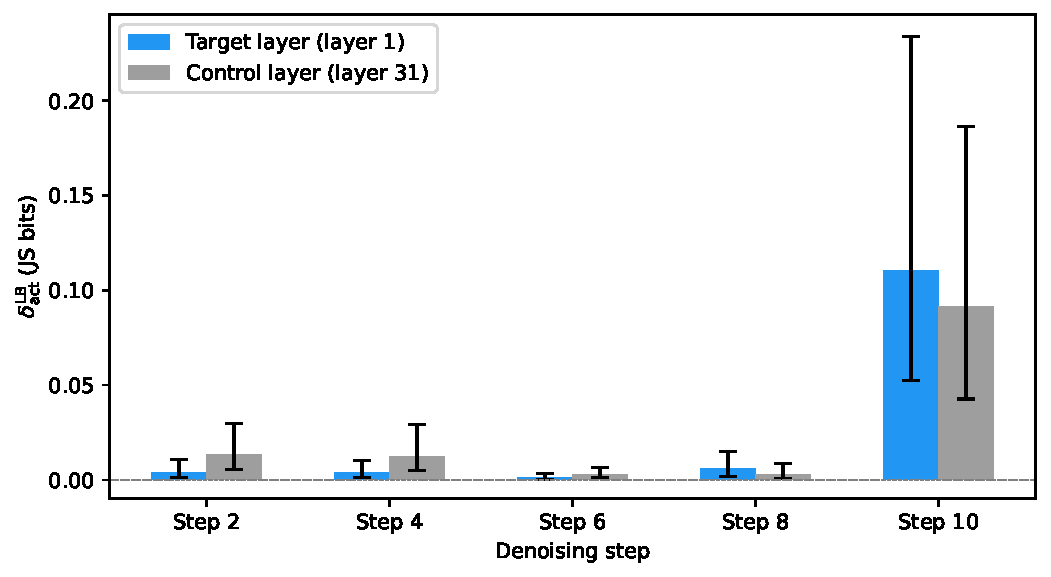
\includegraphics[width=0.62\textwidth]{figures/llada_temporal.pdf}
  \caption{Temporal activation profile for LLaDA-8B-Instruct. Early denoising
  steps have low dynamic certificates; the final action-forming step has a much
  larger certificate for both target and control layers, indicating late-binding
   decision relevance rather than a module-local scratchpad effect.}
  \label{fig:llada-temporal}
  \end{figure}

  The pattern is late-binding. Steps 2--8 remain near the floor for the target
  layer ($0.001$--$0.006$ bits), while step~10 rises to $0.110$ bits with 95\%
  CI $[0.052,0.234]$. The control layer also rises at step~10 ($0.092$ bits, CI
  $[0.043,0.186]$), so the sensitivity is global rather than confined to the
  chosen layer. LLaDA carries hidden capacity throughout denoising; it becomes
  action-relevant when the denoising state binds to a discrete tool choice.

  \subsection{Multi-Agent Private-Report Intervention}
  \label{sec:multi-agent-private-report}

  The multi-agent setting changes the index again. Here the controller delegates
   evidence gathering to a worker, so the worker's private report is not an
  auxiliary scratchpad but an epistemic edge in the decision graph. The worker
  sees a benchmark item and writes a short report; the controller sees only that
   report and chooses one API from \{\texttt{calculator}, \texttt{search}\}. The
   task pool combines $200$ GSM8K arithmetic items~\citep{cobbe2021training} and
   $200$ HotpotQA multi-hop fact questions~\citep{yang2018hotpotqa} with seed
  $42$.

  The main intervention replaces the worker report with a report from the
  opposite task class while holding the controller protocol fixed. A neutral
  replay removes the report content, and a same-class shuffle replaces it with
  another report from the same task class. An oracle-tag condition directly
  names and flips the API label to measure the binary ceiling. For each task and
   condition, the controller is sampled $k{=}8$ times; labels are parsed as
  \{\texttt{calculator}, \texttt{search}, \texttt{invalid}\}; and
  $\mathrm{JS}(P_\text{base},P_\text{condition})$ is averaged with a task-block
  bootstrap.

  \begin{table}[t]
  \centering
  \begin{tabular}{lcc}
  \toprule
  Condition & $\delta_\text{act}^\text{LB}$ (JS bits) & 95\% CI (bits) \\
  \midrule
  Neutral replay & $0.358$ & $[0.324,\ 0.392]$ \\
  Counterfactual evidence & $0.901$ & $[0.873,\ 0.928]$ \\
  Same-class shuffle & $0.084$ & $[0.060,\ 0.109]$ \\
  Oracle tag upper-bound & $1.000$ & $[1.000,\ 1.000]$ \\
  \bottomrule
  \end{tabular}
  \caption{Topological activation profile for the multi-agent deployment.
  Counterfactual evidence nearly saturates the binary action ceiling, while
  same-class shuffling remains much smaller. Hidden communication is therefore
  behaviorally active when the controller has delegated evidence gathering to
  the worker.}
  \label{tab:multi-agent-dynamic}
  \end{table}

  The contrast is topological. In ReAct, the scratchpad matters only when the
  task needs it. In the multi-agent deployment, the controller's decision is
  routed through the private worker report, so the active site is the
  communication edge itself. Same-class variation is local, neutral removal is
  substantial, and counterfactual evidence reaches $0.901$ bits, close to the
  oracle ceiling.

  % ---------------------------------------------------------------------------
  \section{Discussion}
  \label{sec:discussion}
  % ---------------------------------------------------------------------------

  \subsection{One Plot: Capacity, Then Activation}

  The three experiments follow a single logic. Structural budgets map where
  hidden capacity can reside---scratchpad modules, denoising interfaces,
  peer-state edges. Dynamic certificates identify which of those sites affect
  actions. The same scratchpad is dormant on calculator tasks and active on
  planning tasks in ReAct; in LLaDA, action relevance concentrates at the final
  binding step; in the multi-agent deployment, delegation makes the private
  worker report the active edge.

  Effect sizes index deployment topology. Under the same ReAct topology,
  calculator tasks leave the scratchpad dormant while planning tasks produce
  nonzero action-distribution shifts under intervention ($0.0215$ bits, CI
  $[0.0094,0.0410]$) and controlled replay ($0.0163$ bits, CI
  $[0.0124,0.0208]$). The LLaDA final binding step rises to $0.110$ bits; the
  multi-agent counterfactual report edge rises to $0.901$ bits. A hidden channel
   that supplements an already-determined visible trace has low
  $\delta_\text{act}^\text{LB}$; one that carries the decision has high
  $\delta_\text{act}^\text{LB}$. Under this protocol, a claim that an unobserved
   variable causally affects behavior must identify both a channel in
  $\varepsilon_\text{state}^\text{UB}$ and a probe in
  $\delta_\text{act}^\text{LB}$.

  % ---------------------------------------------------------------------------
  \section*{Acknowledgments}
  % ---------------------------------------------------------------------------

  We thank the developers of Qwen2.5 and LLaDA for the open-weight models used
  in the ReAct and diffusion-LM experiments; the creators and maintainers of
  GSM8K and HotpotQA for benchmark data used in the multi-agent setting; and the
   Hugging Face Transformers, PyTorch, NumPy, scikit-learn, NetworkX, and
  Matplotlib communities for the software infrastructure supporting the
  experiments and figures.
  Computations ran on a single Apple M4 Max workstation.

  % ---------------------------------------------------------------------------
  \bibliographystyle{plainnat}
  \bibliography{references}

  % ---------------------------------------------------------------------------
  \section*{NeurIPS Paper Checklist}
  % ---------------------------------------------------------------------------

  \noindent\textbf{1. Claims}\quad Do the main claims made in the abstract and
  introduction accurately reflect the paper's contributions and scope?

  \emph{Answer:} Yes. The abstract and introduction state the dual-certificate
  framework, the structural upper budget (Proposition~\ref{prop:static-ub}), the
  dynamic lower bound (Proposition~\ref{prop:dynamic-lb}), and the experimental
  results that correspond to them. All claims are matched by theoretical
  derivations (\S\ref{sec:static-cert}--\ref{sec:dynamic-cert}) and empirical
  evidence (\S\ref{sec:empirical}).

  \noindent\textbf{2. Limitations}\quad Does the paper discuss limitations of
  the work?

  \emph{Answer:} Yes. Limitations are discussed in several places: the
  observational bottleneck and proxy-estimator bias/variance
  (Appendix~\ref{app:proxy-bias}), the scope of claims (\S\ref{sec:discussion}),
   the conservative nature of the structural budget, and the dependence on
  software-orthogonality assumptions for tightness (\S\ref{sec:static-cert},
  Appendix~\ref{app:netinfo}).

  \noindent\textbf{3. Theory Assumptions and Proofs}\quad Did you state the full
   set of assumptions of all theoretical results, and did you include complete
  proofs of all theoretical results?

  \emph{Answer:} Yes. All assumptions are stated with each proposition (software
   orthogonality in Lemma~\ref{lem:ortho-decomp}, conditional Markov and DPI for
   Proposition~\ref{prop:dynamic-lb}). Complete proofs are given in the main
  text (proof sketches) and in full detail in Appendix~\ref{app:netinfo}.

  \noindent\textbf{4. Experimental Result Reproducibility}\quad Did you provide
  a way to reproduce the experimental results?

  \emph{Answer:} Yes. Detailed experimental protocols are described in
  Appendix~\ref{app:methodology}, including the structural-budget computation
  procedure and the dynamic-certificate estimation steps (proxy, replay,
  intervention, and private-report intervention). The paper references
  implementation README files. Code and data are included in the supplementary
  material.

  \noindent\textbf{5. Open access to data and code}\quad Did you include the
  code, data, and instructions needed to reproduce the main experimental
  results?

  \emph{Answer:} Yes. Code, precomputed results, and reproduction instructions
  are provided in the supplementary material. The experiments use the
  open-weight Qwen2.5-7B-Instruct model (Apache~2.0).

  \noindent\textbf{6. Experimental Setting/Details}\quad Did you specify all the
   training details (e.g., data splits, hyperparameters, how they were chosen)?

  \emph{Answer:} Yes. Experimental details are reported in \S\ref{sec:empirical}
   and Appendix~\ref{app:methodology}: e.g., 5-fold cross-fitted logistic
  regression, trajectory-block bootstrap with 95\% CIs, PCA dimensions, audit
  discretization $Q=256$, perturbation levels, controller sample count $k$, and
  task-pool sampling seed. Hyperparameter choices are motivated and described.

  \noindent\textbf{7. Experiment Statistical Significance}\quad Does the paper
  report error bars suitably and correctly defined or other appropriate
  information about the statistical significance of the experiments?

  \emph{Answer:} Yes. All experimental tables report 95\% confidence intervals
  obtained via trajectory- or task-block bootstrap
  (\S\ref{sec:exp-intervention}--\ref{sec:multi-agent-private-report},
  Appendix~\ref{app:proxy-bias}). Error bars are shown in the appendix proxy
  figure (Figure~\ref{fig:proxy}). The method for calculating CIs is explained
  in the text and Appendix~\ref{app:methodology}.

  \noindent\textbf{8. Experiments Compute Resource}\quad For each experiment,
  does the paper provide sufficient information on the computer resources (type
  of compute workers, memory, time of execution) needed to reproduce the
  experiments?

  \emph{Answer:} Yes. The paper states that all pipelines ran on a single Apple
  M4 Max workstation (\S\ref{sec:empirical}). This indicates the hardware class
  and scale; no GPU-cluster requirements are needed.

  \noindent\textbf{9. Code Of Ethics}\quad Have you read the NeurIPS Code of
  Ethics and ensured that your research conforms to it?

  \emph{Answer:} Yes. The authors have read and adhere to the NeurIPS Code of
  Ethics. The work focuses on safety-oriented auditing of AI agents and does not
   involve human subjects, privacy-sensitive data, or dual-use risks beyond
  those discussed in the paper.

  \noindent\textbf{10. Broader Impacts}\quad If appropriate for the scope and
  focus of your paper, did you discuss potential negative societal impacts of
  your work?

  \emph{Answer:} Yes. The paper develops a framework for auditing AI agents,
  which is inherently aimed at improving transparency and safety. Potential
  dual-use concerns (e.g., adversaries studying the certificates to design
  harder-to-audit systems) are indirectly acknowledged in the discussion of
  limitations and the conservative nature of the bounds
  (\S\ref{sec:discussion}). The overall contribution promotes responsible AI
  deployment.

  \noindent\textbf{11. Safeguards}\quad Do you have safeguards in place for
  responsible release of models with a high risk for misuse (e.g., pretrained
  language models)?

  \emph{Answer:} N/A. The paper does not release any new pretrained models. It
  uses existing open-weight models (Qwen2.5) as-is for auditing experiments
  without modifying or redistributing them.

  \noindent\textbf{12. Licenses}\quad Did you cite the creators and respect the
  license and terms of use of existing assets?

  \emph{Answer:} Yes. The paper cites the model and dataset assets where
  applicable, acknowledges the supporting software communities (Qwen2.5, LLaDA,
  Hugging Face Transformers, PyTorch, NumPy, scikit-learn, NetworkX, and
  Matplotlib; \S\textsuperscript{*}Acknowledgments), and uses
  publicly available assets in accordance with their respective licenses.

  \noindent\textbf{13. New Assets}\quad Are you releasing new assets (datasets,
  code, models), and did you document them properly?

  \emph{Answer:} No. The experimental code and data are provided in the
  supplementary material for review and will be publicly released and documented
  upon acceptance.

  \noindent\textbf{14. Crowdsourcing and Research with Human Subjects}\quad Did
  you use crowdsourcing or conduct research with human subjects?

  \emph{Answer:} N/A. The research does not involve crowdsourcing or human
  subjects.

  \noindent\textbf{15. IRB Approvals}\quad Did you describe potential
  participant risks and obtain Institutional Review Board (IRB) approvals (or an
   equivalent approval/review)?

  \emph{Answer:} N/A. No human subjects research was conducted; therefore, IRB
  approval is not applicable.

  \noindent\textbf{16. Declaration of LLM usage}\quad Does the paper describe
  the usage of LLMs if it is an important, original, or non-standard component
  of the core methods in this research?

  \emph{Answer:} N/A. The LLM (Qwen2.5) serves only as the audit target---it is
  not a component of the proposed auditing method. The auditing framework itself
   (min-cut computation, mutual-information lower bounds, and the
  dual-certificate logic) is independent of any particular language model and
  does not rely on LLMs as a core methodological component.

  \newpage

  \appendix

  % ---------------------------------------------------------------------------
  \section{Network Information Theory Background for
  Proposition~\ref{prop:static-ub}}
  \label{app:netinfo}
  % ---------------------------------------------------------------------------

  \paragraph{Conditional channel capacity.}
  For each unlogged edge $e$ in the time-unrolled DAG $G_t$, the conditional
  capacity $c_e$ is the maximum information that can flow through $e$ under the
  worst-case distribution consistent with the system protocol. It is not an
  empirical average mutual information. It is a structural upper bound read from
   interface specifications: token window length, hidden-dimension size,
  quantization level, and discrete-state cardinality. Concretely, a text channel
   with budget $K$ tokens over vocabulary $\mathcal{V}$ has $c_e \leq K \log
  |\mathcal{V}|$; a vector state of dimension $d$ at quantization $Q$ has $c_e
  \leq d \log Q$; a discrete scheduler with $|\Omega|$ states has $c_e \leq \log
   |\Omega|$. The $K \log |\mathcal{V}|$ form is the maximum-entropy bound
  (uniform over $K$-token sequences); any other distribution gives strictly
  lower entropy. Auditors who can measure the empirical input distribution to a
  particular channel may substitute a tighter bound, which only improves the
  certificate.

  \paragraph{What tightening means.}
  The structural budget remains valid under any replacement $c_e^\star \geq
  I(X_e; Y_e \mid \tilde T_t)$, so tightening is a matter of choosing smaller
  but still defensible per-edge budgets. In practice, this means replacing the
  worst-case $K \log |\mathcal{V}|$ or $d \log Q$ budget with an empirical or
  conditional estimate at the same audit discretization, rather than changing
  the theorem itself.

  \paragraph{Cut-set upper bound and additive decomposition.}
  Let $G_t = (V_t, E_t)$ be the time-unrolled DAG. For a cut $\Omega \subseteq
  V_t$ separating source nodes from a target node, the \emph{induced cut
  capacity} $C_\text{cut}(\Omega)$ is the supremum, over joint input
  distributions $p(X_\Omega \mid \tilde T_t)$, of the directed conditional
  mutual information $I(X_\Omega \to Y_{\Omega^c} \mid \tilde T_t,
  X_{\Omega^c})$. The network-information-theoretic cut-set upper
  bound~\citep{elgamal2011network} states that any information flowing from
  sources in $\Omega$ to a target in $\Omega^c$ is bounded above by
  $C_\text{cut}(\Omega)$, and minimizing over cuts gives the tightest such
  bound. Proposition~\ref{prop:static-ub} applies this bound to the unrecorded
  trace fragment $M_t$. We use the cut-set \emph{upper bound} direction only;
  the network-coding achievability results~\citep{ahlswede2000network}, which
  concern lower bounds on capacity under cooperative coding across the cut, are
  not invoked. The induced capacity $C_\text{cut}(\Omega)$ is in general a
  supremum over joint input distributions and cannot be read directly from
  interface specifications. Lemma~\ref{lem:ortho-decomp} shows that under
  software orthogonality, when the channel laws across the cut factor into
  independent single-edge channels conditional on $\tilde T_t$, the induced
  capacity is bounded above by the sum of per-edge capacities:
  \[
    C_\text{cut}(\Omega) \;\leq\; \sum_{e \in E(\Omega, \Omega^c)} c_e.
  \]
  Corollary~\ref{cor:additive-ub} combines this with
  Proposition~\ref{prop:static-ub} to reduce the certificate computation to a
  discrete minimum-cut problem on $G_t$ with edge capacities $c_e$. This is the
  form used in the structural-budget experiment and in the protocol in
  \S\ref{app:methodology}.

  \paragraph{Formal derivation of Proposition~\ref{prop:static-ub}.}
  The proof in \S\ref{sec:static-cert} has two steps: a trace-gap identity and a
   cut-set bound via $d$-separation. We restate the argument here with the
  $d$-separation step explicit.

  \emph{Step 1: Trace-gap identity.} Let $M_t := T_t \setminus \tilde T_t$. The
  chain rule of conditional entropy gives 
  \[
    H(S_t \mid \tilde T_t) = H(S_t \mid T_t) + I(S_t; M_t \mid \tilde T_t).
  \]
  The first term is $\varepsilon_\text{nominal} = H(S_t \mid T_t)$.

  \emph{Step 2: Cut-set bound via $d$-separation.} Fix a cut $\Omega \in
  \mathrm{Cuts}(U_t \to S_t)$. By the definition of a cut in the time-unrolled
  DAG $G_t$, every directed path from a node in $\Omega$ to $S_t \in \Omega^c$
  must cross at least one edge in $E(\Omega, \Omega^c)$. The causal influence of
   $M_t$ on $S_t$ must be mediated by the cross-cut message stream $(X_\Omega
  \to Y_{\Omega^c})$ together with the boundary state $X_{\Omega^c}$. Formally,
  $M_t$ is $d$-separated from $S_t$ by $(X_\Omega \to Y_{\Omega^c},\,
  X_{\Omega^c})$ conditional on $\tilde T_t$, which yields
  \[
    I(S_t; M_t \mid \tilde T_t) \;\leq\; I\!\left(X_\Omega \to Y_{\Omega^c}
  \;\Big|\; \tilde T_t,\, X_{\Omega^c}\right).
  \]
  By the definition of $C_\text{cut}(\Omega)$ as the supremum of the right-hand
  side over admissible joint input distributions on $X_\Omega$,
  \[
    I(S_t; M_t \mid \tilde T_t) \;\leq\; C_\text{cut}(\Omega).
  \]
  Since this holds for every cut, it holds for the minimum,
  \[
    I(S_t; M_t \mid \tilde T_t) \;\leq\; \min_{\Omega \in \mathrm{Cuts}(U_t \to
  S_t)} C_\text{cut}(\Omega).
  \]
  Combining with Step 1 completes the proof of Proposition~\ref{prop:static-ub}.
   Corollary~\ref{cor:additive-ub} follows immediately by substituting
  Lemma~\ref{lem:ortho-decomp} into each software-orthogonal cut: under
  orthogonality, $C_\text{cut}(\Omega) \leq \sum_{e \in E(\Omega, \Omega^c)}
  c_e$, and the minimum over cuts becomes a discrete min-cut problem on the
  unlogged subgraph with edge capacities $c_e$.

  % ---------------------------------------------------------------------------
  \section{Experimental Protocols}
  \label{app:methodology}
  % ---------------------------------------------------------------------------

  \subsection{Structural Budget Computation Protocol}

  Inputs: deployment architecture specification, logging manifest, and protocol
  budgets (token window sizes, hidden dimensions, quantization levels).
  Procedure: (1)~construct the time-unrolled DAG $G_t$; (2)~partition edges into
   logged and unlogged; (3)~verify software orthogonality
  (Lemma~\ref{lem:ortho-decomp}) or add shared-state edges explicitly to $G_t$
  until orthogonality holds; (4)~assign capacity $c_e$ per unlogged edge using
  the forms in \S\ref{sec:static-cert}; (5)~enumerate reachable cut sets
  $\mathcal{C}_\text{unlogged}$ with a min-cut algorithm after logged edges are
  collapsed to zero residual capacity; (6)~compute
  $\varepsilon_\text{state}^\text{UB} = \varepsilon_\text{nominal} + \min_C
  \sum_{e \in C} c_e$ via Corollary~\ref{cor:additive-ub}.

  For the logging ablation, repeat steps (2)--(6) for the ordered manifests used
   in \S\ref{sec:exp-static}: output-only trace, tool-call trace, router-logit
  trace, summary-buffer trace, and full scratchpad trace. Report the upper-bound
   value and active minimum-cut edges at each level. See
  \texttt{experiments/7.1\_static\_certificate/README.md} for implementation.

  \subsection{Dynamic Certificate Estimation Protocol}

  \paragraph{Proxy certificate.} Inputs: model, task environment, and probe
  family $Z_t^{(k)} = f_k(S_t)$. Steps: (1)~run inference on $N$ trajectories
  and record $(\tilde T_t, Z_t^{(k)}, A_t)$; (2)~train cross-fitted predictors
  $p_\theta(A_t \mid \tilde T_t)$ and $p_\phi(A_t \mid \tilde T_t, Z_t^{(k)})$;
  (3)~compute the cross-entropy difference $\hat I_k = L_\text{trace} -
  L_{\text{trace}+Z^{(k)}}$; (4)~estimate trajectory-block bootstrap intervals;
  (5)~repeat for random, label-permuted, 1-dimensional, 3-dimensional,
  5-dimensional, and full-slice proxies.

  \paragraph{Optional controlled replay certificate.} Inputs: model and two
  controlled execution regimes (wild and replay). Steps: (1)~for each $\tilde
  T_t$, run the same system under wild and replayed missing-state conditions;
  (2)~estimate $\hat\Delta = \hat{\mathrm{JS}}(P_\text{wild}, P_\text{replay}
  \mid \tilde T_t)$; (3)~aggregate over trace slices. This is not output-only
  paraphrase replay; it is valid only under the controlled replay condition in
  \S\ref{sec:replay-cert}.

  \paragraph{Intervention certificate.} Inputs: model, targeted hidden module,
  perturbation budget, and task split. Steps: (1)~inject $\xi_\text{hidden}$ at
  levels $\{0, \sigma_1, \sigma_2, \ldots\}$ while holding $\tilde T_t$ fixed;
  (2)~record $(\xi_\text{hidden}, A_t \mid \tilde T_t)$ pairs; (3)~estimate
  $\hat I(\xi_\text{hidden}; A_t \mid \tilde T_t)$ via conditional
  action-distribution shift for discrete action spaces, or via InfoNCE/MINE for
  continuous action spaces; (4)~repeat on dormant tasks and active tasks under
  the same topology to test whether $\delta_\text{act}^\text{LB}$ changes while
  $\varepsilon_\text{state}^\text{UB}$ remains fixed. The implementation
  persists per-sample argmax actions, tool-token log probabilities, and
  normalized tool-choice probabilities so the aggregate JS rows can be
  recomputed from raw intervention traces.

  \paragraph{Multi-agent private-report certificate.} Inputs: task pool, worker
  model, controller model, and a two-class API space. Steps: (1)~sample $N/2$
  arithmetic tasks and $N/2$ factual-retrieval tasks; (2)~have the worker
  generate a private evidence report under a prompt that forbids direct API
  names and audit each report for leakage; (3)~sample the controller action
  distribution $k$ times under wild, neutral replay, opposite-class report,
  same-class shuffled report, and oracle-tag conditions; (4)~parse actions into
  \{\texttt{calculator}, \texttt{search}, \texttt{invalid}\}; (5)~compute
  per-task JS divergence in bits and task-block bootstrap intervals. The
  oracle-tag contrast is reported only as an upper bound; the main contrast is
  the opposite-class worker-report intervention.

  See the README files for experiments 7.2, 7.3, and 7.6 for implementation.

  % ---------------------------------------------------------------------------
  \section{Proxy Estimator: Bias and Variance}
  \label{app:proxy-bias}
  % ---------------------------------------------------------------------------

  The read-only proxy experiment is a calibration of observational access, not a
   main activation result. On $3{,}000$ tool-selection trajectories (mixed
  calculator/search/email/calendar/weather), we record $\tilde T_t$
  (embedding-layer representation), $Z_t$ (layer-24 tool-logit projection), and
  $A_t$. The CE-diff $\hat I = \mathcal{L}(A_t\mid\tilde T_t) -
  \mathcal{L}(A_t\mid\tilde T_t,Z_t)$ is estimated via 5-fold cross-fitted
  logistic regression with trajectory-block bootstrap.
  Table~\ref{tab:proxy-results} reports the resolution ablation: random,
  1/3/5-dim PCA, and full 10-dim proxy.

  The $d{=}5$ PCA proxy recovers $0.0317$ bits ($1.4\%$ of the $\log_2 5 = 2.32$
   bit ceiling) with CI excluding zero on the mixed-task distribution. The
  magnitude reflects an \emph{observational bottleneck}: when the baseline
  predictor achieves near-perfect accuracy, the ceiling $H(A_t \mid \tilde T_t)
  \approx 0$ caps any read-only proxy. Intervention and replay avoid this
  bottleneck by changing the missing-state condition while holding the visible
  transcript fixed.

  The dormant/active proxy split should be read as an estimator-noise
  diagnostic. On calculator tasks (dormant scratchpad), $H(A_t \mid \tilde T_t)
  = 0$ empirically, yielding $\delta_\text{act}^\text{LB} = 0$ trivially. On
  planning tasks (active scratchpad), the proxy row is positive in point
  estimate but has a wide CI that straddles zero. We therefore do not use the
  read-only proxy as the main body evidence for active scratchpad use; the
  causal intervention and controlled replay in \S\ref{sec:exp-intervention}
  supply that evidence.

  \begin{table}[ht]
  \centering
  \begin{tabular}{lcc}
  \toprule
  Proxy & CE-diff (bits; nats) & 95\% CI (bits) \\
  \midrule
  \multicolumn{3}{c}{\textit{Resolution ablation (mixed task)}} \\
  random & $-0.0007$; $-0.0005$ & $[-0.0012,-0.0003]$ \\
  $d=1$ PCA & $+0.0065$; $+0.0045$ & $[+0.0053,+0.0078]$ \\
  $d=3$ PCA & $+0.0250$; $+0.0173$ & $[+0.0225,+0.0273]$ \\
  $d=5$ PCA & $+0.0317$; $+0.0220$ & $[+0.0273,+0.0358]$ \\
  full $(10\text{-dim})$ & $+0.0183$; $+0.0127$ & $[+0.0134,+0.0229]$ \\
  \midrule
  \multicolumn{3}{c}{\textit{Dormant/active split (d=64 PCA, L2-regularized)}}
  \\
  calculator (dormant) & $0.0000$; $0.0000$ & $[0,0]$ \\
  planning (active) & $+0.0412$; $+0.0286$ & $[-0.0725,+0.1386]$ \\
  \bottomrule
  \end{tabular}
  \caption{Read-only proxy calibration. Top: resolution ablation on the mixed
  tool-selection dataset. Bottom: dormant/active split. The active-task row is
  reported honestly as an estimator-noise diagnostic because its confidence
  interval straddles zero; causal replay/intervention supplies the body evidence
   for active scratchpad use. Negative random-control CE-diff is a finite-sample
   artifact near the noise floor and is clipped to zero when interpreted as a
  lower-bound certificate.}
  \label{tab:proxy-results}
  \end{table}

  \begin{figure}[ht]
  \centering
  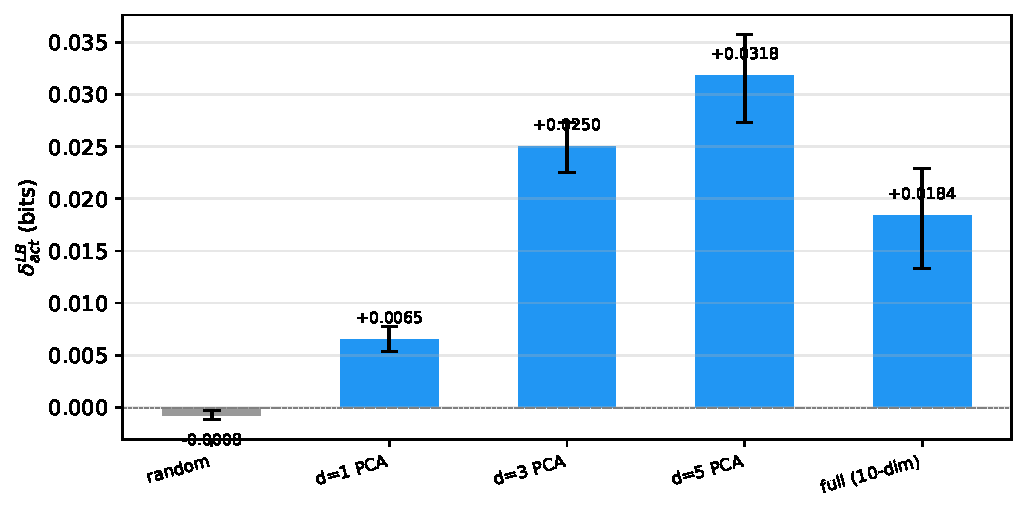
\includegraphics[width=0.55\textwidth]{figures/proxy_ablation.pdf}
  \caption{Proxy resolution ablation. $\delta_\text{act}^\text{LB}$ increases
  monotonically through $d{=}5$ PCA. The random proxy sits near zero (estimator
  leakage check). Error bars are 95\% trajectory-block bootstrap CIs.}
  \label{fig:proxy}
  \end{figure}

  The CE-diff estimator $\hat I = L(\tilde T_t) - L(\tilde T_t, Z_t)$
  lower-bounds $I(Z_t; A_t \mid \tilde T_t)$, but three bias sources and two
  variance sources matter in practice.

  \paragraph{Bias sources.}
  (1)~\emph{Proxy coarsening:} $Z_t = f(S_t)$ discards information in $S_t$ not
  captured by $f$, so $I(Z_t; A_t \mid \tilde T_t) \leq I(S_t; A_t \mid \tilde
  T_t)$. The gap is the coarsening loss.
  (2)~\emph{Restricted predictor class:} Logistic regression or shallow MLPs may
   not reach the Bayes-optimal predictor, so the CE-diff underestimates the true
   conditional MI.
  (3)~\emph{Finite-sample bias:} With finite $N$, the cross-entropy on held-out
  folds is an upward-biased estimate of the population CE, and the difference of
   two such estimates carries residual bias. Cross-fitting mitigates but does
  not eliminate this.

  \paragraph{Variance sources.}
  (1)~\emph{Trajectory sampling:} The $N$ observed trajectories are a finite
  sample from the deployment distribution. Block bootstrap over trajectories
  estimates the resulting CI.
  (2)~\emph{Proxy dimension:} Higher-dimensional proxies carry more information
  but increase predictor variance. The PCA ablation in
  Table~\ref{tab:proxy-results} shows this trade-off: $d{=}5$ outperforms both
  $d{=}3$ and the full 10-dimensional proxy.

  \paragraph{Mean squared error.}
  Decomposing $\text{MSE} = (\text{bias})^2 + \text{variance}$, the proxy
  certificate is a conservative lower bound: positive bias (underestimation) is
  safe for the audit (it never overstates $\delta_\text{act}$), while variance
  widens the CI but does not shift the point estimate.

  \paragraph{Sampling noise and temperature.}
  Increasing decoding temperature can raise $H(A_t \mid \tilde T_t)$, but
  independent sampler noise is not a certificate amplifier. It changes the
  audited policy and can reduce $I(Z_t; A_t \mid \tilde T_t)$ when the added
  action variation is unrelated to the hidden state proxy. A temperature sweep
  is therefore a calibration of a randomized deployment policy, not a substitute
   for proxy quality or causal access. We do not use temperature injection for
  the main proxy certificate; the synthetic experiment instead injects
  hidden-state stochasticity with known ground truth.

  % ---------------------------------------------------------------------------
  \section{Synthetic Ground-Truth Validation}
  \label{app:synthetic}
  % ---------------------------------------------------------------------------

  To test whether the certificates recover known hidden influence, we construct
  a synthetic agent whose hidden-state entropy and decision relevance are
  controlled by design. A binary hidden variable $H \sim \text{Bern}(0.5)$
  injects influence of strength $\beta_h$ into the action logits; the
  unlogged-channel capacity $c_H = H(H) = 1$ bit is known. We run both the
  static min-cut ($\varepsilon_\text{state}^\text{UB}=1$ bit) and the proxy
  CE-diff estimator on $1{,}000$ trajectories at five influence levels.

  \begin{figure}[ht]
  \centering
  
\includegraphics[width=0.55\textwidth]{figures/synthetic_gt.pdf}
  \caption{Synthetic ground-truth. $\varepsilon_\text{state}^\text{UB}$ (blue)
  equals the true $H(S_t \mid \tilde T_t) = 1$ bit.
  $\delta_\text{act}^\text{LB}$ (red) tracks the true $I(S_t; A_t \mid \tilde
  T_t)$ from below, with negative values at low $\beta_h$ reflecting estimator
  variance near the noise floor.}
  \label{fig:synthetic}
  \end{figure}

  Fig.~\ref{fig:synthetic} shows $\varepsilon_\text{state}^\text{UB} = 1$ bit
  matches the true hidden entropy (the bound is tight when there is no redundant
   unlogged capacity). The dynamic lower bound $\delta_\text{act}^\text{LB}$
  tracks the true conditional MI from below at all tested influence levels
  ($\beta_h \geq 1$); negative CE-diff values at $\beta_h=0$ reflect
  finite-sample variance around a near-zero true MI.

  The Qwen deployment has a near-deterministic baseline that suppresses the
  proxy signal ($H(A_t \mid \tilde T_t) \approx 0$). The synthetic environment
  instead injects controlled stochasticity ($H = 1$ bit of hidden-state
  entropy). Without that observational bottleneck, the proxy certificate
  $\delta_\text{act}^\text{LB}$ tracks the true conditional-MI curve from below
  in the tested range. The validation shows that the proxy certificate can
  become tight when structural capacity is behaviorally active \emph{and} the
  observational ceiling permits detection.

  % ---------------------------------------------------------------------------
  \section{Tightening the Static Certificate}
  \label{app:static-tightening}
  % ---------------------------------------------------------------------------

  The reported structural budget is intentionally conservative. Its role is to
  upper-bound the residual hidden-state entropy from deployment topology alone,
  so the default budgets in \S\ref{sec:static-cert} are worst-case interface
  capacities rather than empirical information estimates.

  \paragraph{Empirical and conditional budgets.}
  A tighter deployment-specific certificate can replace the worst-case budget
  $c_e$ on each unlogged edge by an empirically justified budget $c_e^\star$.
  For a text channel, one option is a high-confidence upper bound on $H(X_e \mid
   \tilde T_t)$; when the visible history strongly constrains the missing input,
   a conditional form such as $H(X_e \mid \tilde T_t, \mathcal H_t)$ can be
  smaller still. For quantized vector states, the analogous replacement is an
  empirical entropy or rate-distortion budget at the same audit discretization.
  These substitutions do not alter the min-cut proof: they only change the edge
  weights used by Corollary~\ref{cor:additive-ub}.

  \paragraph{Graph refinement.}
  If two apparent channels share latent state, naive edge-wise additivity can
  double-count the same information. The remedy is to refine the time-unrolled
  DAG so that the shared state appears as an explicit node or edge family, then
  recompute the min-cut on the refined graph. This usually tightens the
  certificate more reliably than trying to compensate with ad hoc weight
  corrections.

  \paragraph{Reporting policy.}
  For review and deployment, report a ladder of certificates: worst-case
  structural, empirical-marginal, and empirical-conditional. The first is the
  theorem-backed safety baseline. The latter two are optional tightening modes
  and should be reported only when the underlying measurements are defensible.

  \end{document}

  ---
  The paper was already technically clean — no Tier 1 vocabulary violations, low
   hedging density, and precise empirical language. The 10 targeted edits
  removed rhetorical delay sentences, fixed two odd metaphors ("visible to a
  single scalar," "reused across settings"), tightened the bridge paragraph
  before Proposition 1, compressed the §5 intro by one sentence, and gave the
  Discussion a synthetic opening instead of a restatement. All theorem numbers,
  CI bounds, citations, and labels are unchanged.
